\documentclass[14pt]{extbook}
\usepackage{multicol, enumerate, enumitem, hyperref, color, soul, setspace, parskip, fancyhdr} %General Packages
\usepackage{amssymb, amsthm, amsmath, latexsym, units, mathtools} %Math Packages
\everymath{\displaystyle} %All math in Display Style
% Packages with additional options
\usepackage[headsep=0.5cm,headheight=12pt, left=1 in,right= 1 in,top= 1 in,bottom= 1 in]{geometry}
\usepackage[usenames,dvipsnames]{xcolor}
\usepackage{dashrule}  % Package to use the command below to create lines between items
\newcommand{\litem}[1]{\item#1\hspace*{-1cm}\rule{\textwidth}{0.4pt}}
\pagestyle{fancy}
\lhead{Module6}
\chead{}
\rhead{Version C}
\lfoot{7334-5530}
\cfoot{}
\rfoot{test}
\begin{document}

\begin{enumerate}
\item{
Describe the zero behavior of the zero $x = -9$ of the polynomial below.\[ f(x) = -2(x - 4)^{9}(x + 4)^{7}(x + 9)^{3}(x - 9)^{2} \]} \newpage
\item{
Write an equation that \textit{could} represent the graph below.
\begin{center}
    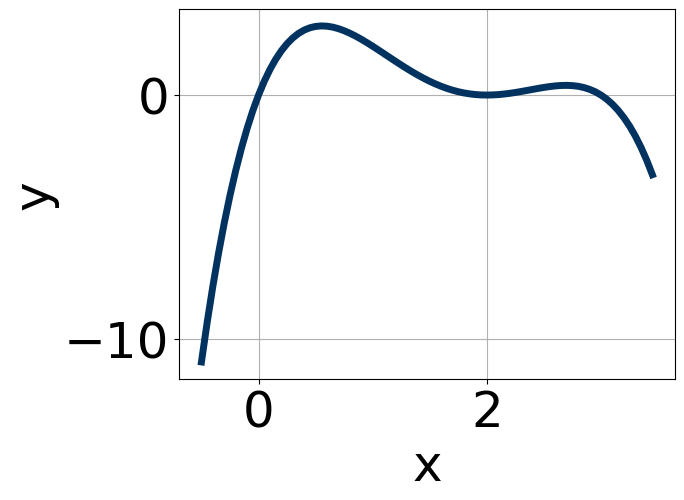
\includegraphics[width=0.5\textwidth]{../Figures/polyGraphToFunctionC.png}
\end{center}
} \newpage
\item{
Construct the lowest-degree polynomial given the zeros below.\[ 1, \frac{7}{4}, \text{ and } \frac{5}{3} \]} \newpage
\item{
Describe the zero behavior of the zero $x = 9$ of the polynomial below.\[ f(x) = 2(x - 7)^{6}(x + 7)^{4}(x + 9)^{8}(x - 9)^{7} \]} \newpage
\item{
Construct the lowest-degree polynomial given the zeros below.\[ 7, \frac{-7}{3}, \text{ and } 4 \]} \newpage
\item{
Describe the end behavior of the polynomial below.\[ f(x) = 7(x + 6)^{3}(x - 6)^{6}(x - 3)^{3}(x + 3)^{3} \]} \newpage
\item{
Construct the lowest-degree polynomial given the zeros below.\[ 2 - 2 i \text{ and } 2 \]} \newpage
\item{
Write an equation that \textit{could} represent the graph below.
\begin{center}
    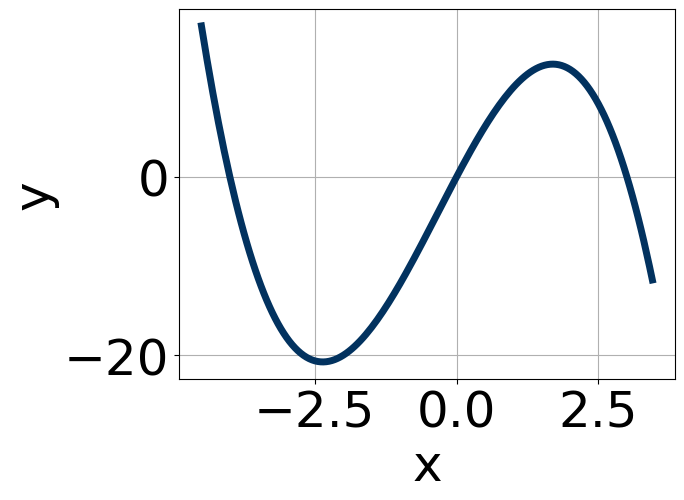
\includegraphics[width=0.5\textwidth]{../Figures/polyGraphToFunctionCopyC.png}
\end{center}
} \newpage
\item{
Construct the lowest-degree polynomial given the zeros below.\[ -2 - 4 i \text{ and } 3 \]} \newpage
\item{
Describe the end behavior of the polynomial below.\[ f(x) = 7(x + 5)^{4}(x - 5)^{5}(x + 9)^{2}(x - 9)^{3} \]} \newpage
\end{enumerate}

\end{document}